\section{Demarche Expérimentale}

\begin{figure}[h]
    \centering
    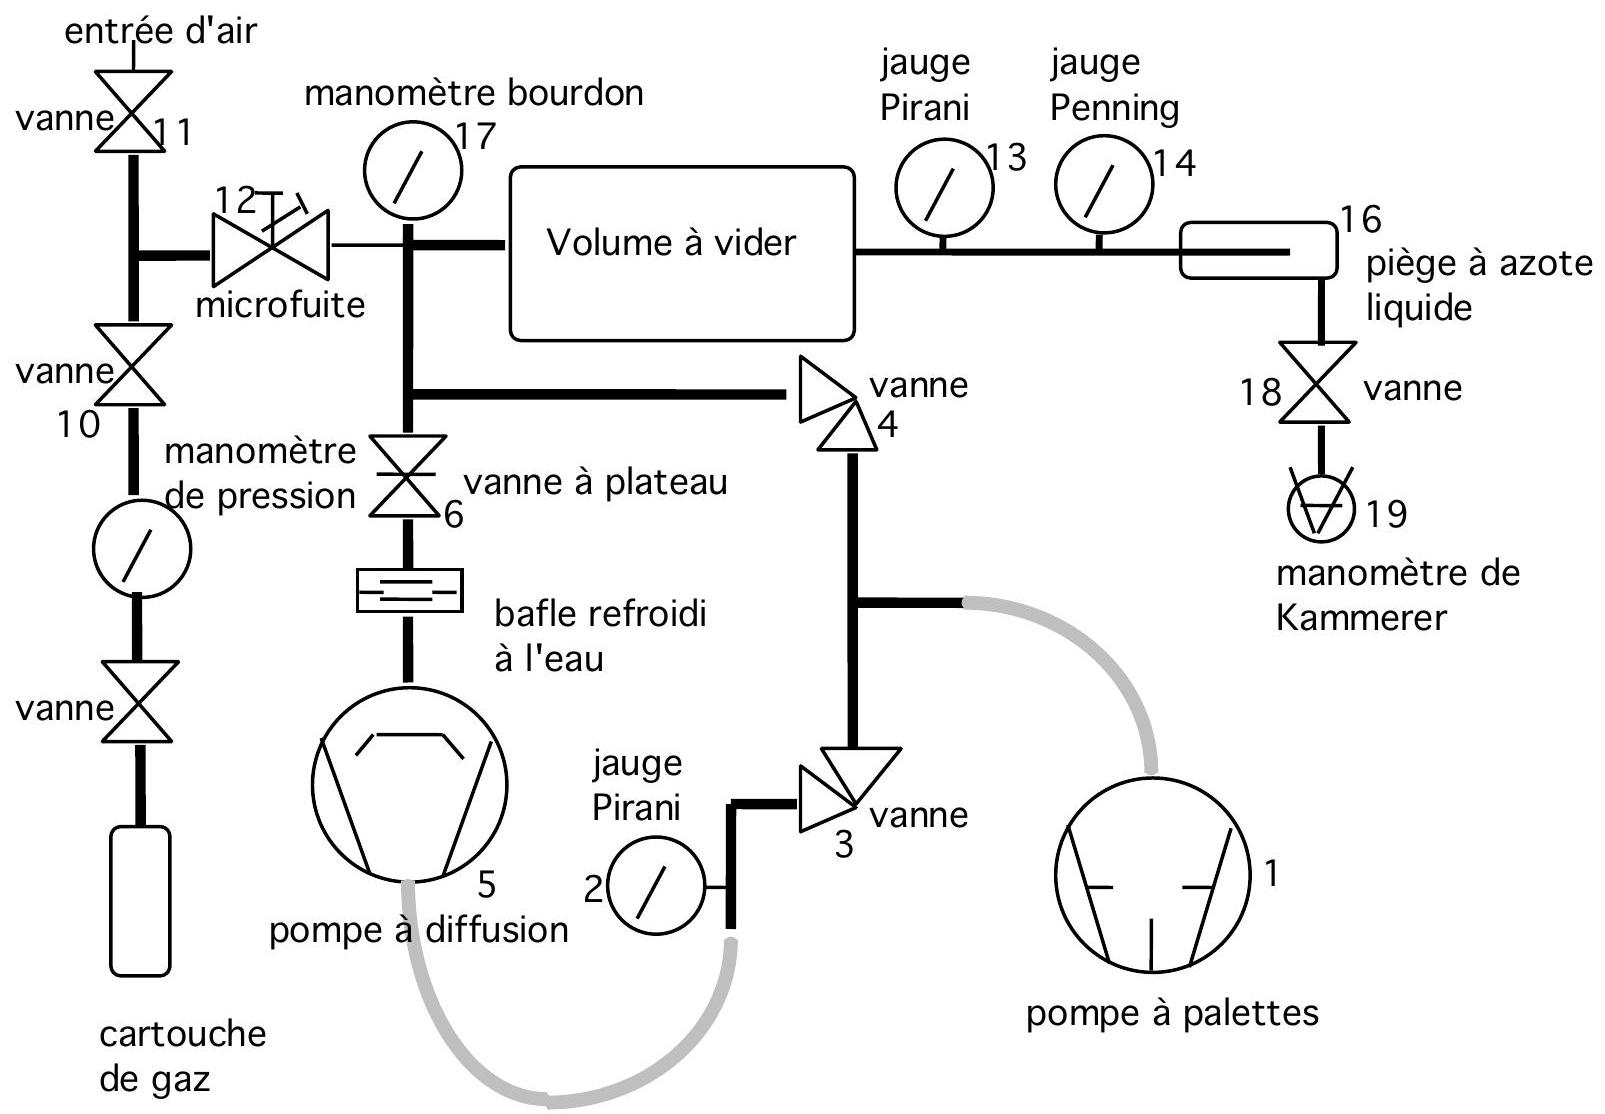
\includegraphics[width=0.95\textwidth]{figures/montage_cinetique.png}
    \caption{Montage pour mesurer la cinétique des pompes}
    \label{fig:montagecinetique}
\end{figure}

\paragraph*{Cinétique de pompage}
Pour mesurer le changement de pression en fonction du temps dans la chambre à vide pour les pompes primaires et secondaires le plus précisément possible, les manomètres sont filmés pendant une durée de 15 \unit{\minute}. Un shéma du montage est donné à la \autoref{fig:montagecinetique}. La pression à la fin de ces 15 \unit{\minute} est utilisée pour estimer les valeurs de la pression limite \(p_\textrm{lim,1}\) de la pompe primaire et \(p_\textrm{lim,2}\) de la pompe secondaire.

Les pompes étudiées dans cette expérience sont:

\begin{itemize}
    \item La pompe à palettes permettant de créer un vide primaire (\(1 - 10^{-3}\) \unit{\milli\bar}), fonctionnant avec un système de compression - expulsion à l'aide d'une vanne rotative.
    \item La pompe à diffusion permettant de créer un vide secondaire (\(10^{-3} - 10^{-7}\) \unit{\milli\bar}), fonctionnant en transferant l'énergie des molécules de vapeur d'huile dans les molécules d'air.
\end{itemize}

\begin{minipage}{\textwidth}
\begin{wrapfigure}{R}{0.5\textwidth}
    % \centering
    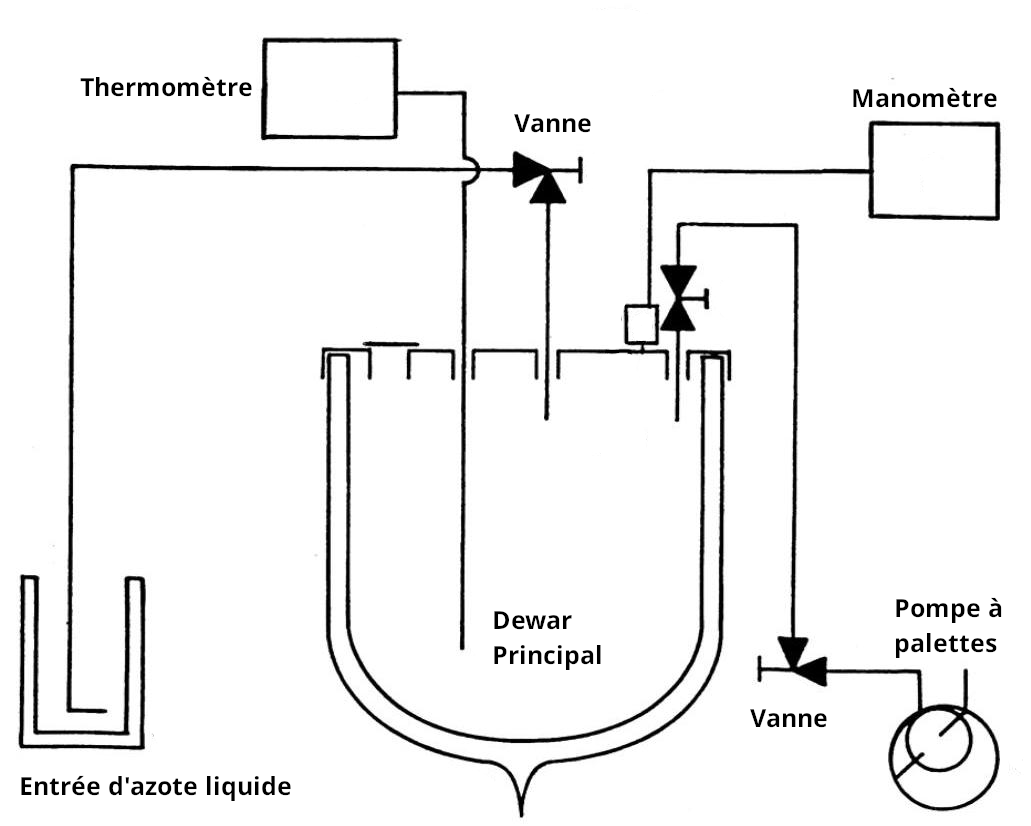
\includegraphics[width=\linewidth]{figures/montage_point_triple.png}
    \caption{Montage pour mesurer le point triple de l'azote et les courbes de transformation de phase}
    \label{fig:montagepointtriple}
\end{wrapfigure}

Trois manomètres permettant de mesurer différentes gammes du vide sont utilisés:

\begin{itemize}
    \item Manomètre de Bourdon: domaine \(> 10\) \unit{\milli\bar}
    \item Jauge de Piranni: domaine de \(100\) à \(10^{-3}\) \unit{\milli\bar}
    \item Jauge de Penning: domaine de \(10^{-3}\) à \(10^{-7}\) \unit{\milli\bar}
\end{itemize}

\paragraph*{Point triple de l'azote}
La mesure du point triple de l'azote est réalisée à l'interieur d'un dewar permettant d'avoir une meilleure isolation de l'exterieur. L'azote est aspiré grâce au vide créé par une pompe à palettes dans le dewar principal. L'expérience est filmée pour relever la température et la pression simultanément, permettant d'obtenir les courbes de transition de phase. Le montage sur place n'avait pas d'agitateur.
\end{minipage}

